\documentclass[aspectratio=169]{beamer}
\usetheme{metropolis}
\usepackage[utf8]{inputenc}
\usepackage{tikz}
\usetikzlibrary{positioning,fit,backgrounds,arrows.meta}
\usepackage{booktabs}
\usepackage{array}

\definecolor{talkteal}{HTML}{1F6F78}
\definecolor{talkcoral}{HTML}{C05746}
\definecolor{talkgold}{HTML}{D1A344}
\setbeamercolor{palette primary}{bg=talkteal,fg=white}
\setbeamercolor{frametitle}{bg=talkteal,fg=white}
\setbeamercolor{progress bar}{fg=talkcoral,bg=talkteal!20}
\setbeamercolor{alerted text}{fg=talkcoral}

\title{Bias, ESS, and Debiasing in Massively-Parallel Importance Sampling}
\subtitle{An empirical audit of \texttt{alan}'s MP-IS, and two early follow-ups}
\author{}
\date{}

\begin{document}

\maketitle

\begin{frame}{Outline}
  \tableofcontents
\end{frame}

% =============================================================
\section{Why look at this}
% =============================================================

\begin{frame}{Where this started}
  A colleague's reaction to \texttt{alan}'s massively-parallel importance
  sampling (MP-IS):
  \begin{quote}
    \itshape ``\dots probably not going to beat HMC per se, what with the
    posterior estimates being biased by self-normalization, but mostly seems
    to do a reasonable job of trying to catch up to it eventually.''
  \end{quote}
  \vfill
  \begin{center}
    \alert{Is that actually true?} Let's measure it, on a model small enough
    that we know the exact answer.
  \end{center}
\end{frame}

\begin{frame}{MP-IS in one slide}
  \begin{columns}[T]
    \begin{column}{0.52\textwidth}
      \textbf{The idea:}
      \begin{itemize}
        \item Draw $K$ candidate values (``particles'') per latent variable,
          instead of one.
        \item Reweight them to approximate the true posterior.
        \item Exploit conditional independence across \texttt{Plate}s so
          this costs $O(K)$ per latent, not $O(K^{\text{\#latents}})$.
      \end{itemize}
      No claim of exactness --- it's still importance sampling, just a much
      more sample-efficient version of it.
    \end{column}
    \begin{column}{0.44\textwidth}
      \begin{center}
      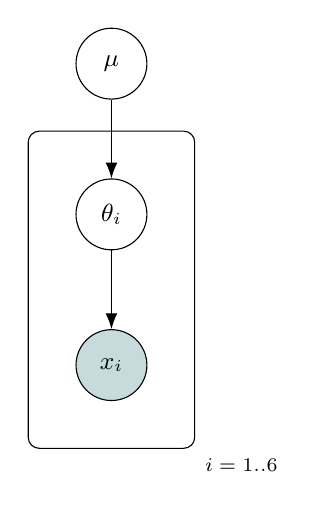
\begin{tikzpicture}[
          node distance=10mm and 8mm,
          var/.style={circle,draw,minimum size=9mm,font=\small},
          obs/.style={circle,draw,fill=talkteal!25,minimum size=9mm,font=\small}
        ]
        \node[var] (mu) {$\mu$};
        \node[var,below=of mu] (theta) {$\theta_i$};
        \node[obs,below=of theta] (x) {$x_i$};
        \draw[-{Latex[length=2mm]}] (mu) -- (theta);
        \draw[-{Latex[length=2mm]}] (theta) -- (x);
        \begin{scope}[on background layer]
          \node[draw,rounded corners,fit=(theta)(x),inner sep=6mm,label={[font=\scriptsize]south east:$i=1..6$}] {};
        \end{scope}
      \end{tikzpicture}
      \end{center}
      \begin{center}\scriptsize the toy model used throughout this talk\end{center}
    \end{column}
  \end{columns}
\end{frame}

% =============================================================
\section{Does MP-IS actually beat HMC?}
% =============================================================

\begin{frame}{Setup: a model small enough to know the truth}
  \begin{itemize}
    \item $\mu \sim \mathcal{N}(0,1)$, $\ \theta_i \mid \mu \sim
      \mathcal{N}(\mu,1)$, $\ x_i \mid \theta_i \sim \mathcal{N}(\theta_i,0.7)$,
      $i=1..6$, $x$ observed.
    \item Linear-Gaussian $\Rightarrow$ \textbf{exact} posterior available
      (Hessian of the log joint) --- no need to trust any single method.
    \item Compared: \texttt{alan}'s MP-IS, plain (``Global'') self-normalized
      IS at the same $K$, and a hand-rolled HMC sampler validated against the
      exact posterior.
  \end{itemize}
\end{frame}

\begin{frame}{Headline result}
  \begin{center}
    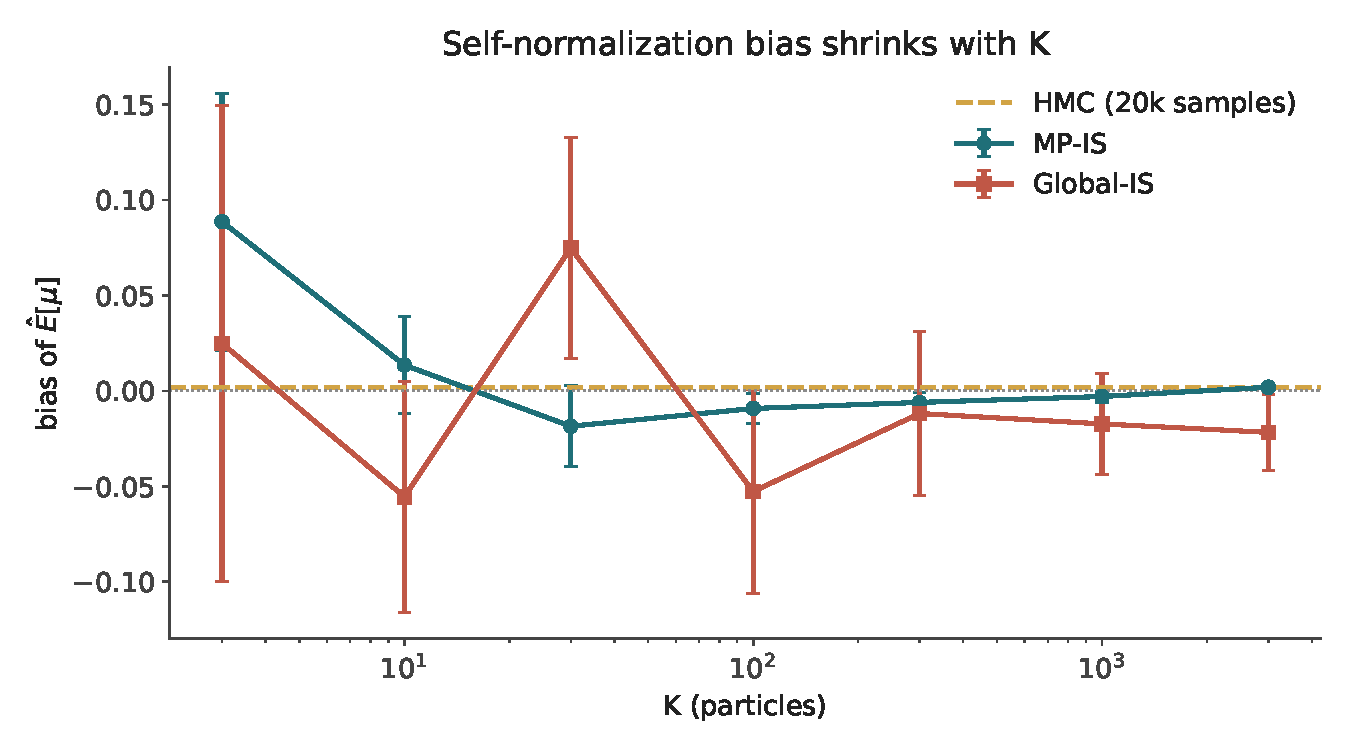
\includegraphics[width=0.92\textwidth]{figures/bias_vs_K.pdf}
  \end{center}
\end{frame}

\begin{frame}{Takeaways}
  \begin{itemize}
    \item The colleague was right: MP-IS \alert{is} biased at small $K$, and
      the bias \alert{does} shrink and catch up to HMC's own (tiny) bias.
    \item The sign flip between $K{=}10$ and $K{=}30$ is the classic
      signature of finite-sample self-normalization bias --- not just noise.
    \item Global-IS is consistently 5--10$\times$ worse than MP-IS at the
      \emph{same} $K$ across the whole sweep. Plate structure is doing real
      work.
  \end{itemize}
\end{frame}

% =============================================================
\section{A bug hunt}
% =============================================================

\begin{frame}{A hand-rolled reimplementation didn't match}
  To dig further into \emph{why} MP-IS is biased, I rebuilt its computation
  by hand for this toy model, so I could see every intermediate number.
  \vfill
  \begin{center}
    \alert{It didn't reproduce \texttt{alan}'s own output.} Not by a rounding
    amount --- by enough to matter.
  \end{center}
  \vfill
  Every individual $\log p$ / $\log q$ term matched. The mismatch was in how
  the pieces get combined.
\end{frame}

\begin{frame}{Two ways to reduce a plate}
  \begin{columns}[T]
    \begin{column}{0.48\textwidth}
      \begin{alertblock}{Order A (what I assumed)}
        Sum the plate's 6 log-densities together first, \\
        \emph{then} do one reduction over the shared $K$ particles.
      \end{alertblock}
    \end{column}
    \begin{column}{0.48\textwidth}
      \begin{block}{Order B (what \texttt{alan} does)}
        Reduce over $K$ particles \emph{separately for each of the 6 plate
        elements}, then sum those 6 already-reduced results.
      \end{block}
    \end{column}
  \end{columns}
  \vfill
  These are genuinely different computations --- the reduction \texttt{alan}
  uses (log-sum-exp) doesn't distribute over a sum.
\end{frame}

\begin{frame}{Order B is the correct one}
  \begin{itemize}
    \item Given $\mu$, the six $\theta_i$'s are \alert{conditionally
      independent}.
    \item A sum over a product of independent terms factors exactly into a
      product of independent sums.
    \item So each plate element is free to pick whichever of its $K$
      particles best explains \emph{its own} observation --- a real,
      quantifiable extra bit of Rao--Blackwellization that plate structure
      buys you for free.
  \end{itemize}
  \vfill
  \small Rebuilt by hand under Order B: matches \texttt{alan}'s ELBO and
  posterior mean exactly, to float32 precision.
\end{frame}

% =============================================================
\section{Effective sample size}
% =============================================================

\begin{frame}{How many of the K particles are actually doing work?}
  Kish's effective sample size, for a normalized weight vector:
  \[
    \text{ESS} = \frac{1}{\sum_k w_k^2} \qquad (\text{always} \le K)
  \]
  \texttt{alan} exposes this \emph{per latent variable}, from the marginal
  posterior it already computes --- not something added for this talk.
\end{frame}

\begin{frame}{ESS results}
  \begin{center}
    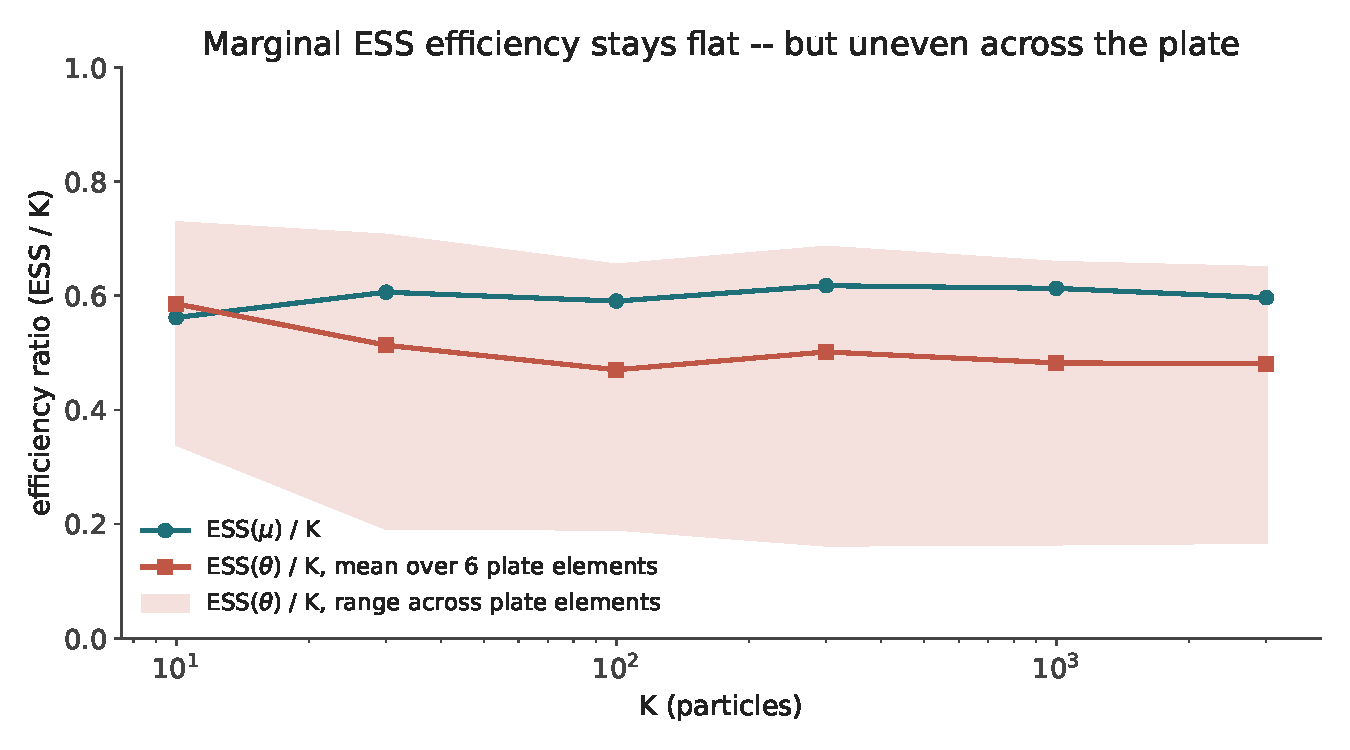
\includegraphics[width=0.92\textwidth]{figures/ess_vs_K.pdf}
  \end{center}
\end{frame}

\begin{frame}{What the spread means}
  \begin{itemize}
    \item Efficiency (ESS/K) for $\mu$ stays flat at $\approx 0.6$ across the
      whole range tested --- more particles doesn't relatively help or hurt.
    \item $\theta$'s efficiency is uneven: at $K{=}3000$, one plate element
      has ESS $\approx$ 504, another $\approx$ 1948 --- roughly a
      $4\times$ gap, from the \emph{same} $K$.
    \item \alert{Flag for later:} that unevenness turns out to matter a lot
      for one of the follow-ups at the end of this talk.
  \end{itemize}
\end{frame}

% =============================================================
\section{Jackknife bias correction}
% =============================================================

\begin{frame}{Can we just correct the bias?}
  \textbf{Delete-one jackknife}, the classical fix for this exact kind of
  bias:
  \begin{enumerate}
    \item Compute the estimate normally, using all $K$ particles.
    \item Recompute it $K$ times, each time leaving one particle out.
    \item Extrapolate: $\hat\theta_{\text{jack}} = K\hat\theta -
      (K-1)\overline{\hat\theta_{-i}}$.
  \end{enumerate}
  No new machinery --- just re-weighted averaging of numbers already
  computed.
\end{frame}

\begin{frame}{Jackknife results}
  \begin{center}
    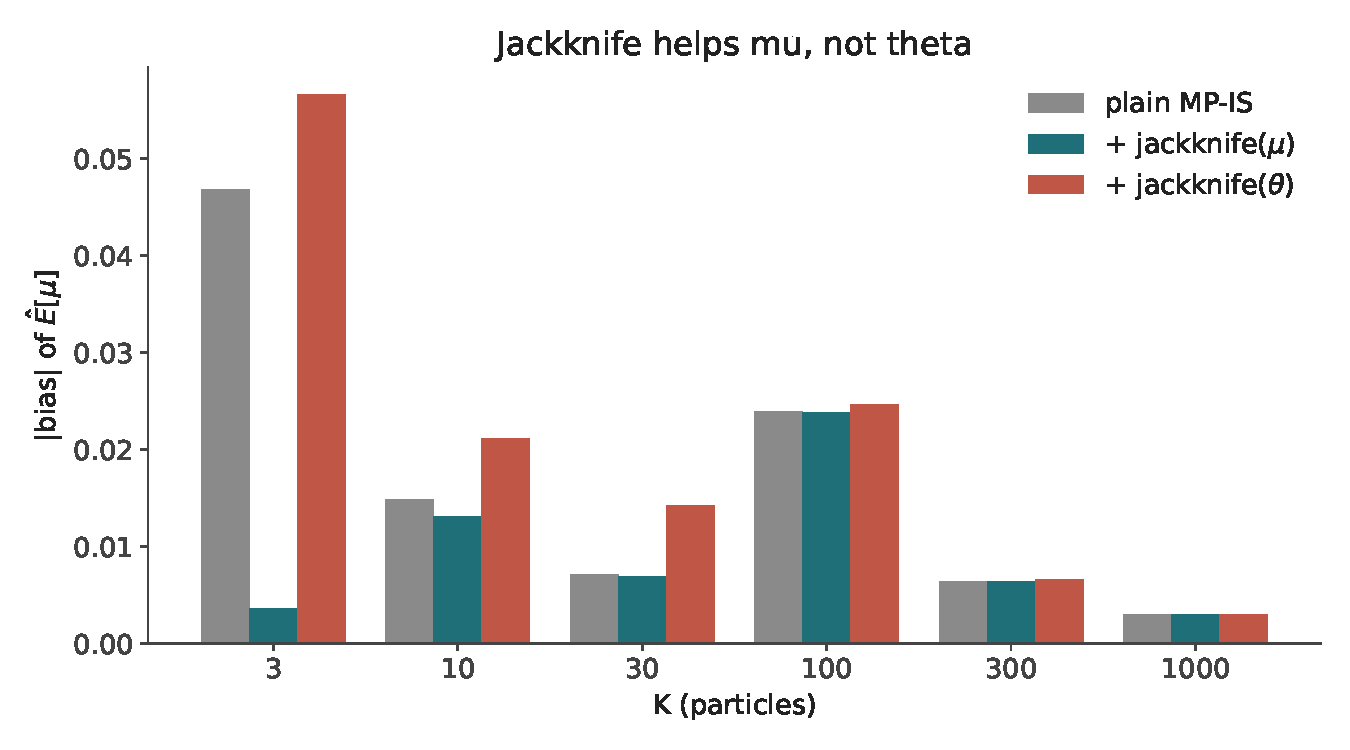
\includegraphics[width=0.92\textwidth]{figures/jackknife_bias.pdf}
  \end{center}
\end{frame}

\begin{frame}{Why $\mu$ but not $\theta$}
  \begin{itemize}
    \item $\mu$ enters the computation through one flat, linear ratio ---
      exactly the textbook shape jackknife theory is derived for.
    \item $\theta$ enters through a \alert{nested} reduction (Order B, from
      earlier): a log-sum-exp \emph{inside} another ratio.
    \item Classical jackknife theory has no mechanism to cancel bias through
      that extra layer of nonlinearity --- and empirically, it doesn't.
  \end{itemize}
  \vfill
  \small A structural rule, not a coincidence: jackknife the \emph{outer},
  flat-ratio part of an estimate; don't bother with the nested, per-plate
  part.
\end{frame}

% =============================================================
\section{Where things stand}
% =============================================================

\begin{frame}{Summary so far}
  \begin{itemize}
    \item MP-IS \emph{is} biased at small $K$, and does converge toward
      HMC-level accuracy --- confirmed, not just assumed.
    \item The bug hunt uncovered a real, previously undocumented fact about
      how \texttt{alan}'s plate reduction works (Order B).
    \item ESS is bounded by $K$ and uneven across plate replicates ---
      quantified, not just suspected.
    \item Jackknife helps, but only for flat/outer reductions --- a precise,
      structural rule for when to bother with it.
  \end{itemize}
\end{frame}

% =============================================================
\section{Further work}
% =============================================================

\begin{frame}{Two follow-up questions}
  \begin{enumerate}
    \item Jackknife couldn't fix $\theta$'s bias. \alert{Is there a
      debiasing method that isn't limited to flat ratios?}
    \item All of the above is still approximate. \alert{Can we get an exact
      posterior out of this same K-particle machinery?}
  \end{enumerate}
  \vfill
  Both are early, toy-model-only prototypes --- not yet integrated into
  \texttt{alan} itself. Included here as a look at what's next.
\end{frame}

\begin{frame}{BR-SNIS: debiasing via a Markov chain}
  Cardoso et al.\ 2022. Instead of one fixed pool of $K$ samples:
  \begin{itemize}
    \item Keep a \emph{running} candidate: at each step, it joins $K{-}1$
      fresh proposal draws.
    \item Pick a new running candidate from that pool, weighted by
      importance weight.
    \item This defines an exact Markov chain targeting the true posterior
      for any $K \ge 2$.
  \end{itemize}
  Bias is driven down by \alert{chain length}, not by needing $K \to
  \infty$ --- a fundamentally different lever than jackknife's.
\end{frame}

\begin{frame}{BR-SNIS: what we found}
  \begin{itemize}
    \item Run flat, over the whole $(\mu,\theta)$ joint: \alert{loses to
      plain MP-IS} --- it ignores the plate's conditional independence, so
      it's $\sim$13$\times$ worse on $\theta$ at matched compute.
    \item Run instead on $\mu$'s already plate-reduced ratio (mirroring what
      jackknife did): competitive with jackknife at matched cost, and
      \alert{doesn't inherit jackknife's variance blow-up at tiny $K$.}
  \end{itemize}
  \vfill
  \small Lesson: general-purpose debiasing has to be pointed \emph{at} the
  structure MP-IS already exploits, not used as a replacement for it.
\end{frame}

\begin{frame}{Particle Gibbs: towards an exact posterior}
  \begin{itemize}
    \item MP-IS gives an \alert{unbiased estimator of the marginal
      likelihood} --- exactly the ingredient Particle MCMC needs for exact
      inference.
    \item \textbf{Particle Gibbs:} pin one full trajectory as a
      ``reference'' that survives every resampling step, by construction ---
      the rest of the particles resample normally.
    \item Needs a genuinely \emph{sequential} model to demonstrate (the toy
      model above is flat, not sequential) --- prototyped instead on a
      small linear-Gaussian state-space model with a closed-form (Kalman
      filter) ground truth.
  \end{itemize}
\end{frame}

\begin{frame}{The catch: reference-trajectory stickiness}
  \begin{center}
    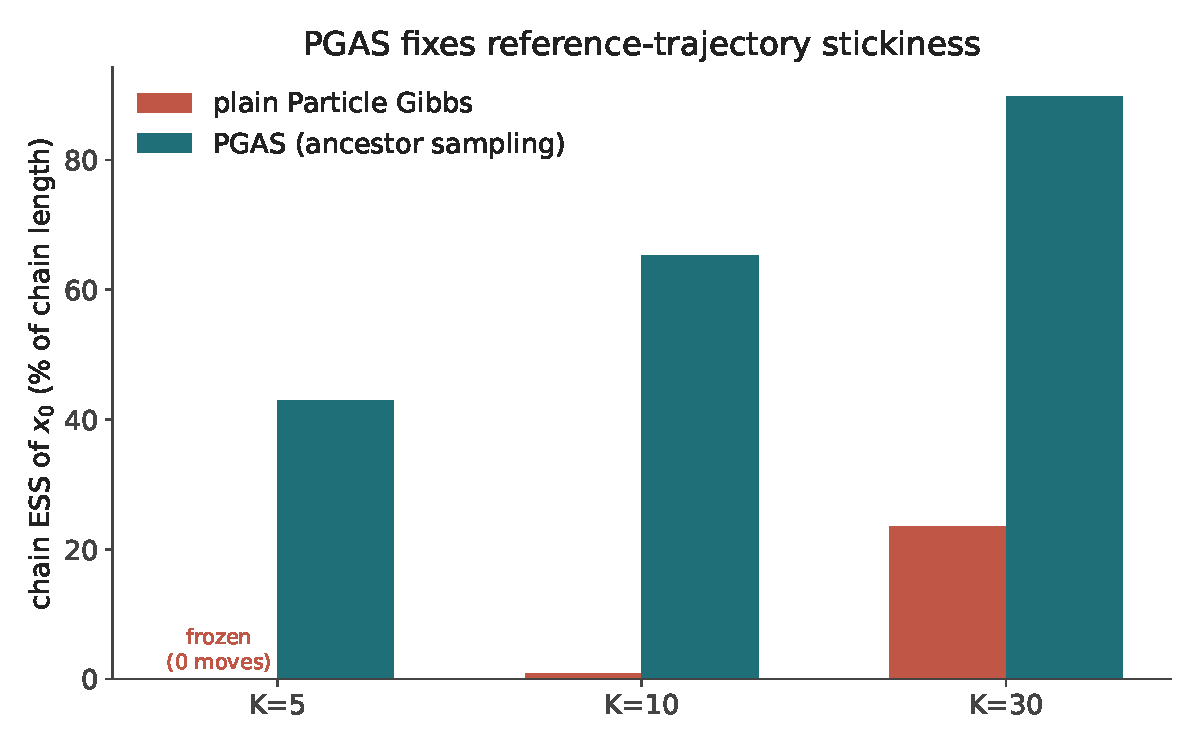
\includegraphics[width=0.85\textwidth]{figures/pg_mixing.pdf}
  \end{center}
  \small At $K{=}5$, plain Particle Gibbs' reference trajectory
  \alert{never moves at all} across 1800 iterations. Ancestor sampling
  (PGAS) fixes it: 74$\times$ better mixing at $K{=}10$.
\end{frame}

\begin{frame}{Why this isn't a surprise}
  This connects directly back to the ESS finding from earlier: uneven
  per-replicate weight degeneracy in MP-IS was already a concrete warning
  sign that plain Particle Gibbs would mix slowly on a model like this.
  \vfill
  \begin{center}
    \alert{Ancestor sampling (PGAS) is now treated as a near-term priority,
    not an optional extra, once real \texttt{alan} integration starts.}
  \end{center}
\end{frame}

\begin{frame}{Where this leaves the design}
  \begin{itemize}
    \item Both prototypes are validated on toy models with closed-form
      ground truth, deliberately \emph{before} touching \texttt{alan}'s
      core sampling code.
    \item Neither is integrated into \texttt{alan} yet --- that's the next,
      more invasive piece of work (\texttt{Plate.py} / \texttt{Sampler.py}).
    \item Both findings are written up and cross-linked into the design doc
      for whoever picks this up next.
  \end{itemize}
\end{frame}

% =============================================================
\section*{Wrap-up}
% =============================================================

\begin{frame}{Summary}
  \begin{itemize}
    \item MP-IS's bias-vs-HMC behavior, measured directly and confirmed.
    \item A real bug in a hand-rolled comparison led to a genuine finding
      about how \texttt{alan}'s plate reduction works.
    \item ESS and jackknife give precise, structural (not just empirical)
      answers about where bias correction does and doesn't help.
    \item Two early prototypes (BR-SNIS, Particle Gibbs/PGAS) point at what
      comes next, with concrete numbers already in hand to prioritize the
      work.
  \end{itemize}
\end{frame}

\begin{frame}[standout]
  Questions
\end{frame}

\end{document}
